\section{Design}
In this section, we present our proposed design for the sensor node, remote server, and gateway. We present this design only after thoroughly performing background research related the Air Quality Index, researching various hardware and software engineering standards, and exploring various potential components. This design combines the information that was collected in previous sections along with our defined requirements and specifications. In order to fully detail our design, we will be both describing our and design as well as including relevant hardware schematics and software flowcharts and diagrams. These will assist in the clarification and understanding of our design.

\importsubsection{embedded}
\importsubsection{server-software}
\importsubsection{gateway}
\importsubsection{server}
\importsubsection{power}
\importsubsection{microcontroller-sensor}

\subsection{Microcontroller and Sensor System}
This section will look at the overall design of the LoRa-E5 MCU and the three main atmospheric sensors in the Aether nodal system. The MCU in the Aether node will use I2C communication protocol to communicate with the sensors and gateway module. Each node is equipped with a Sensirion PM sensor, a Renesas ZMOD4510 sensor, and a Bosch BME688 sensor. The particulate matter sensor is capable of detecting both particulate matter 2.5 PM2.5, and particulate matter 10 (PM10). Renesas' ZMOD4510 sensor is equipped with non-selective nitrogen dioxide (NO2) measurement capabilities with a selective measurement of ozone (O3) as well. The Bosch BME sensor gives the Aether node the flexibility to measure multiple types of gases including Volatile Organic Compounds (VOCs), volatile sulfur compounds (VSCs) and other gases such as carbon monoxide and hydrogen in addition to pressure, temperature & humidity sensor through AI and machine learning models. The MCU will be connected to an antenna on the outside of the enclosure to communicate through the LoRa-WAN network.

\subsubsection{LoRa-E5 MCU}
The ultrlow power LoRa-E5 (STM32WLE5JC) will be the micro-controller responsible for providing long-range wireless communication from the nodes to the gateway. It's a Ultra-Thin Profile Fine Pitch Ball Grid Array (UFBGA) with 73 ball arrays and a 28 pin layout. The chip is powered through VCC Pin 1 which takes 3.3V from the main power rail. Pins PB15 and PA15 are the micro-controller's serial clock and serial data I2C pins which are used to communicate with the sensors in the system. The respective pins on each sensor will be connected to PB15 and PA15 so sensor data can be read at defined intervals. Pin 15 is the RFIO pin which will be connected to the antenna. Additionally, 3 GPIO pins were used to read the 3 status states of the battery charge controller. Pin 21 (PA9) is connected to the MCP73871 PG pin which indicates the system is receiving power. GPIO pin 13 (PC0) on the micro-controller is connected to pin 8 (STAT1/LBO) on the MCP73871 which indicates to the micro-controller when the battery output is low or the system is charging. The third GPIO used is pin 20 (PB10) on the micro-controller which is connected to pin 7 (STAT2) on the MCP73871 which indicates to the micro-controller when the battery has been fully  charged. The nodes will have LEDs to indicate battery status to the users in addition to having the ability to remotely monitor battery status through the LoRa micro-controller. 

The next two pins connected on the micro-controller deal with the USB communication interface. As discussed before, this micro-controller is not equipped with the ability to communicate directly through USB. Once the USB-to-UART conversion circuit was designed the TX and RX outputs on the USB-to-UART bridge were connected to 2 GPIO pins on the micro-controller. Pin 10 (PB6) is responsible for taking USB TX data and Pin Pin 9 (PB7) takes in USB RX output. The TX/RX pins are responsible for transmitting and receiving USB data. Pin 12 (PC1) on the micro-controller is a GPIO pin dedicated to the SHDN pin for the boost converter that takes the Li-Io battery as an input and outputs a consistent 5V for the PM sensor. The micro-controller will be responsible for initiating a low-power mode state for the nodal system which shuts down the PM sensor remotely as on of the means to conserve power. Lastly, pin PB3 is an MCU GPIO configured as an EXTI (external interrupt) source. This pin is responsible for detecting when the USB source is connected and instructs the micro-controller to wake up. 
\subsubsection{Bosch BME688 Sensor}
The Bosch BME688 detects Volatile Organic Compounds (VOCs) and Volatile Sulfur Compounds (VSCs) and other gases through the use of sophisticated AI embedded in the system and machine learning algorithms. This sensor comes in a 3.0 mm x 3.0 mm x 0.93 mm metal lid 8-pin LGA. Aether's Bosch BME688 sensor supports two digital communication interfaces: I2C and SPI. As previously discussed, I2C will be the main source of communication in our overall design and the BME688 I2C interface can support the Standard, Fast and High Speed modes of the sensor. To activate the I2C interface on the Bosch sensor, the VDDIO pin 6 is connected the chip select status (CSB) pin 2. To power the sensor, VDD pin 8 is connected to the 3.3V power rail and tothe VDDIO pin. Both VDD and VDDIO are paired with decoupling capacitors connected to ground to help oppose fast changes of voltage. The pins dedicated to the I2C communication interface are serial clock (SCL), data (SDA), and slave address LSB (SDO). Because SDI is bi-directional, it is connected to VDDIO via a pull-up resistor. Once the I2C communication interface is activated on the chip, the next step is to make the appropriate connections to the LoRa micro-controller. The serial data input (SDI) pin 3 is directly connected to the serial data (SDA) pin 6 on the micro-controller. The serial clock (SCL) pin on the Bosch sensor is connected to pin 5 on the micro-controller. The SDO pin on the sensor is tied to ground for the default slave address.  
\paragraph{}

\subsubsection{Renesas ZMOD4510 Sensor}
The ZMOD4510 is a 12-pin LGA assembly with dimensions of 3.0 ×3.0 ×0.7mm equipped with an I2C communication protocol. This is the sensor responsible for detecting nitrogen dioxide and ozone in the the Aether node. The serial clock and serial data pins for the I2C interface on the sensor module will go connected to the respective pins on the LoRa micro-controller, pins 5 and 6. VDD is the voltage supply for the ZMOD4510 and VDDH is the voltage supply for the integrated heater in the ZMOD4510. The VDDIO pin is the voltage supply for I/O-interface in ZMOD4510. These 3 voltage supply pins will all be connected to the 3.3V power rail. Pin 3 on the ZMOD4510 is the interrupt pin on the sensor. This pin will read HIGH when a measurement is running and LOW when a measurement has finished. It will be connected to GPIO pin 11 on the LoRa micro-controller. The VSS pins for the ZOMOD are the sensors ground references and will therefore be tied to ground. The ZMOD is equipped with a RES function on pin 11. This is an  active low pin connected to the 3.3V power rail via a 10KOhm pull-up resistor. 

\subsubsection{Sensirion Particulate Matter Sensor}
Aether's SPS30 sensor will be responsible for collecting particulate matter data for the node. Unlike the other 2 sensors discussed, the SPS30 will not be soldered directly onto the main PCB board. The interface is a 5-pin JST connector located at the side of the sensor opposite to the air inlet/outlet. Because this sensor relies on a built-in fan to collect ambient particle samples, it will be placed at the very edge of the inner housing for the node. A JST female wire harness plug will then be used to connect the sensor to the 5-pin ZHR-5 connector on the main PCB board. SPS30 offers both UART and I2C communication. To activate the I2C communication protocol on the SPS30 sensor, the select (SEL) pin must be tied directly to ground. This particulate matter sensor operates with a 5V input, which is the reason we needed to design a 5V power rail in Aether's power schematic through a boost converter. The VDD pin on the SPS30 is the supply voltage pin that will be powered by this 5V rail. Pins 2 and 3 are the SDA and SCL pins on the SPS30, respectively. The I2C pins will be connected to the respective pins on the LoRa micro-controller and tied to 10kOhm pull-up resistors connected to the 3.3V power rail. A 3.3V input was used instead of 5V for the SDA and SCL pins because the pins are LVTTL 3.3V compatible. Using 3.3V instead of 5V for the I2C pins ensures no over-voltage damage is done to the micro-controller since it operates under the 5V range. The overall schematic design for the Aether node MCU and sensor system can be seen in Figure \ref{fig:MCU_Sensor}

\begin{sidewaysfigure}
    \centering
    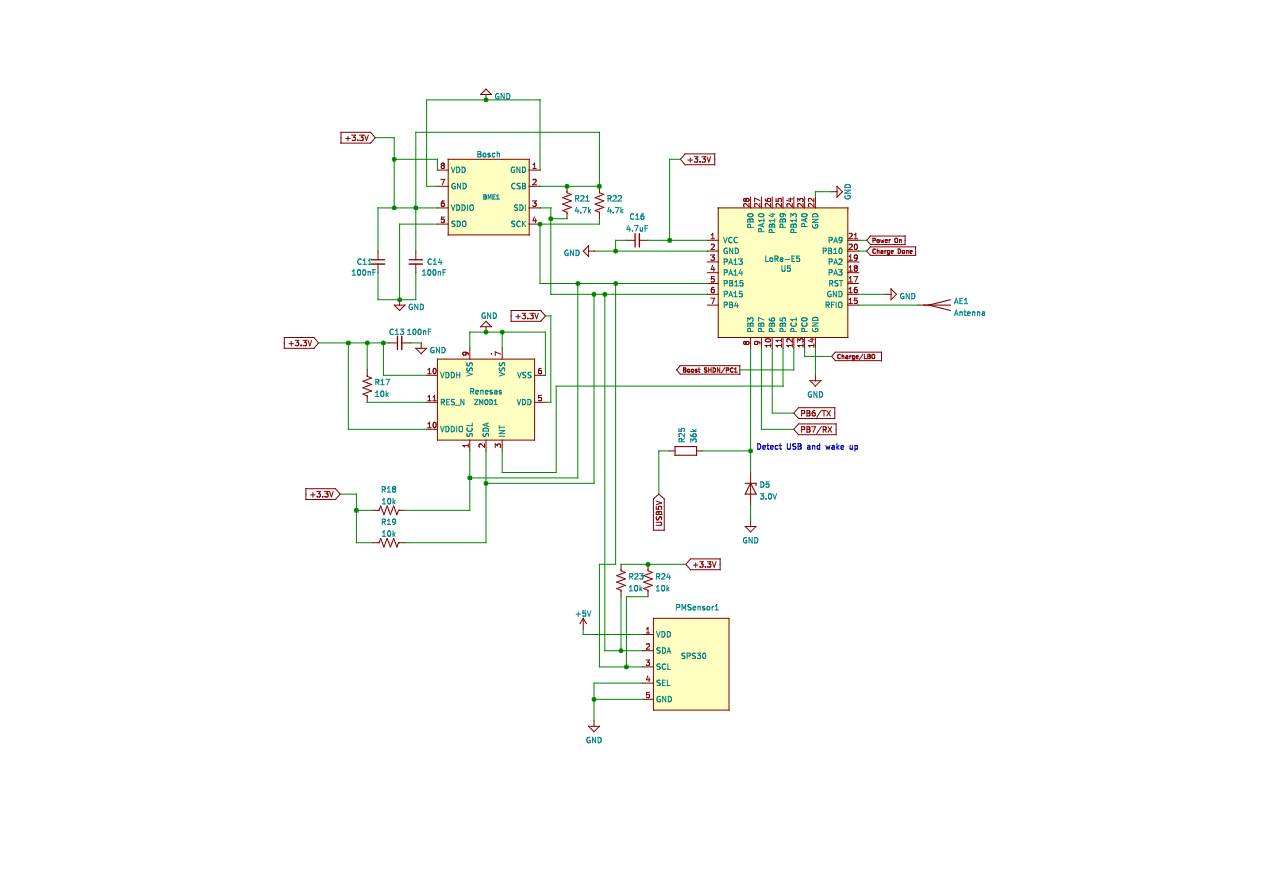
\includegraphics[scale=0.5]{figures/MCU_Schematic.jpg}
    \caption{Aether Node MCU and Sensor System Schematic}
    \label{fig:MCU_Sensor} 
\end{sidewaysfigure}

\importsubsection{mechanical}
\subsection{Design Summary}
Aether's power design for the node consist of two main power inputs: a 6V solar panel and a USB-C input. The node will be able to operate using either of these inputs and when one is connected it will be simultaneously powering the system while charging the battery. Before a USB-C port could be connected to the system, protection circuitry needed to be designed to prevent against ESD and EMI damage. Additionally, since the LoRa micro-controller can not communicate directly through USB protocol, a USB-to-UART bridge IC needed to be implemented in the design to allow for proper communication between USB and the LoRa module. The next step in the power design for the Aether node was having a charge controller IC capable of taking 2 varying power inputs and efficiently charge the battery. A major challenge to this design was finding a charge controller IC that would not demand excessive current from the solar panel and continuously charge and discharge the battery, decreasing the overall system efficiency. The MCP73871 is capable of using as much current as the solar panel can output without reaching its drop out voltage. In the Aether power design, when the solar panel cannot efficiently meet system load demands, the MCP73871 charge controller will take the remaining necessary current from the Li-Io battery to feed the load. If the USB is used as the power input, the charge controller will efficiently charge the battery and the USB input will be used to power the system. Since the LoRa module and most of the sensors in the system operate at a 3.3V range, a linear voltage drop out (LDO) regulator was needed at the MCP73871 output to design a 3.3V power line for the system. The particulate matter sensor in the node requires a 5V input so a boost converter was used, taking the battery as an input to output a consistent 5V power rail. Additionally, a therm-resistor is connected to a pin on the MCP73871 to monitor battery temperature and ensure the battery is not charge under unsafe conditions. 

For the Aether MCU and sensor subsystem, the 3 main sensors in the Aether node are connected to the LoRa-E5 MCU and communicate through I2C protocol. The Bosch BME688 sensor and Renesas' ZMOD4510 sensor operate using the 3.3V power rail while the SPS30 Particulate Matter sensor uses the 5V power input from the boost converter. The sensors are configured to I2C communication and the respective SCD and SCL pins are connected to the LoRa module. An antenna which will be used for the LoRa receiver is connected to the MCU. Several GPIO pins on the LoRa module are used for communicating with the system, including USB communication, battery status, and remote shutdown of the SPS30 sensor for low-power mode operation. Protection features against ESD and EMI were only needed to be implemented for the USB-to-UART interface since all 3 sensor came with built in circuit protection features. Additionally, an MCU GPIO pin is configured as an EXTI (external interrupt) source to detect USB input and wake up the micro-controller.
 